\part{Honeypot}
\section{Honeypot}

\begin{frame}
	\partpage
\end{frame}

%%%%%%%%%%%%%%%%%%%%%%%%%%%%%%%%%%%%%%%%%%%%%%%%%%%%%%%%%%%%%%%%%%%%%%%%%%%%%%%
\begin{frame}
	\frametitle{Definition and goals}
	
	A honeypot is a \textbf{ICT resource} used for monitoring, detecting and analyzing attacks. It has no production value, no real sensible data. 
	
	\smallskip

	Can be classified by its implementation (virtual or physical), purpose (prevention, detection, research) and level of interaction (low, middle, high) in particular:
	
	\medskip

	\textbf{Low-interaction honeypots} simulate only some aspects of the system, while limiting the ability of the attacker. More easy to deploy but can get a limited amount of information.
	
	\medskip
	
	\textbf{High-interaction honeypots} based on a real OS, the attackers gets full access to the system and can be compromised completely (with an higher risk). Harder to deply and manage but can get a full overview of the attackers.
	
	\medskip

  Many OpenSSH honeypot solutions exists but due to their popularity they are easy to detect.
  
	\smallskip

  An high-interaction custom honeypot was chosen in order to maximize the information gathered from the attackers.
  	
\end{frame}
%%%%%%%%%%%%%%%%%%%%%%%%%%%%%%%%%%%%%%%%%%%%%%%%%%%%%%%%%%%%%%%%%%%%%%%%%%%%%%%


%%%%%%%%%%%%%%%%%%%%%%%%%%%%%%%%%%%%%%%%%%%%%%%%%%%%%%%%%%%%%%%%%%%%%%%%%%%%%%%
\begin{frame}
	\frametitle{Honeypot structure and strategy}
	
	\footnotesize
	
  Credentials are leaked in two different ways.
  
  \smallskip

  For a client backdoor is enough to \textbf{log into the honeypot server}. 
  
  \smallskip

  More complicate is for a daemon backdoor, one solution is to \textbf{install the daemon backdoor} on the honeypot server, 
  log in with a safe client and remove the backdoor, in order to simulate the backdoor detection in the attacker eyes.

  \smallskip

  \begin{center}    
  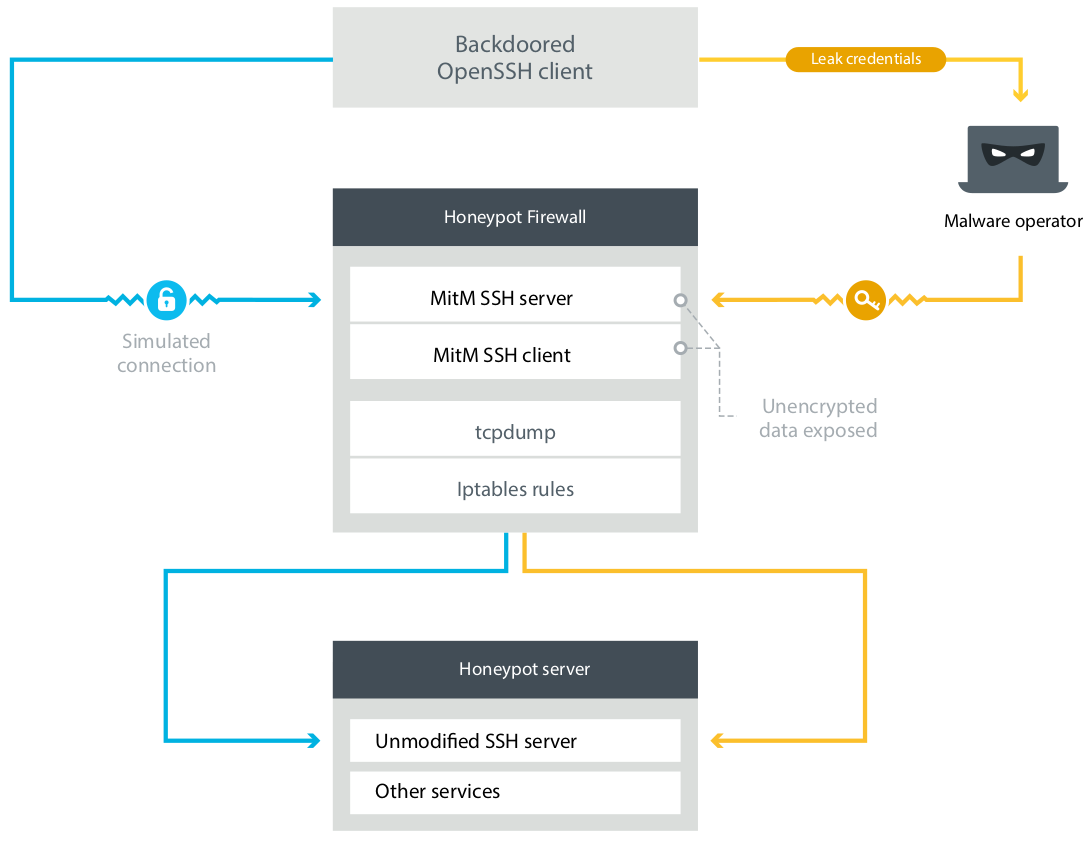
\includegraphics[width=0.5\textwidth]{images/honeypot_infrastructure}
  \captionof{figure}{Honeypot infrastructure}
  \end{center}

\end{frame}
%%%%%%%%%%%%%%%%%%%%%%%%%%%%%%%%%%%%%%%%%%%%%%%%%%%%%%%%%%%%%%%%%%%%%%%%%%%%%%%


%%%%%%%%%%%%%%%%%%%%%%%%%%%%%%%%%%%%%%%%%%%%%%%%%%%%%%%%%%%%%%%%%%%%%%%%%%%%%%%
\begin{frame}
	\frametitle{Observed interaction: Minban}
	
	Both client and server backdoors were available, of course the backdoor client was used to leak the credentials.
	
	\smallskip
	
	The attackers behing the backdoor logged in to the honeypot after few hours of leaking and thanks to the architecture the commands executed on the server were logged.
	
	\smallskip
	
  \begin{center}    
  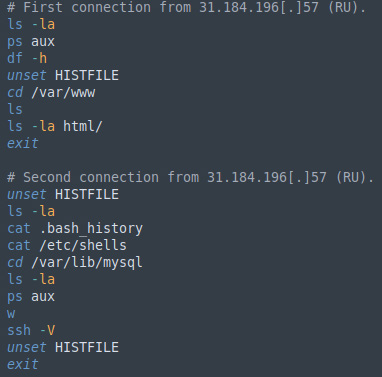
\includegraphics[width=0.25\textwidth]{images/minban}
  \captionof{figure}{Attackers command captured for Minban}
  \end{center}
  
	\smallskip
	
  Attackers logged in manually from a \textbf{Russian IP address}, try to clean command history, check some files and finally \textbf{check the version of OpenSSH binary}.  

\end{frame}
%%%%%%%%%%%%%%%%%%%%%%%%%%%%%%%%%%%%%%%%%%%%%%%%%%%%%%%%%%%%%%%%%%%%%%%%%%%%%%%


%%%%%%%%%%%%%%%%%%%%%%%%%%%%%%%%%%%%%%%%%%%%%%%%%%%%%%%%%%%%%%%%%%%%%%%%%%%%%%%
\begin{frame}
	\frametitle{Observed interaction: Borleias}
	
	More interesting the results of the Borleias backdoor: the attackers first logged into the honeypot in less than 24 hours and repeat for \textbf{more than 10 times} withing four days.
	
	\smallskip
	
	\begin{itemize}
	  \item The attackers used \textbf{Tor} to login, in order to not leave trace.
	  \item A classic version of the OpenSSH client was used to connect.
	  \item They managed to get the credential leaked in the Mimban operations: this means that there is a \textbf{connection between the two backdoors} (maybe same operators or the credentials were sold somewhere).
	  \item Some basic checks at beginning then more interesting operations in the few days later, in particular they drop a \textbf{new version of the backdoor}.
	  \item Gather all the information about the server, exfiltrate them and clean all the command history.
	  \item \textbf{Meticulous attention to details} (check of running process, timestamps of files, logged-in users between the execution of each command, ...)
	\end{itemize} 
	
\end{frame}
%%%%%%%%%%%%%%%%%%%%%%%%%%%%%%%%%%%%%%%%%%%%%%%%%%%%%%%%%%%%%%%%%%%%%%%%%%%%%%%
